\documentclass[12pt,a4paper]{article}
\special{papersize=210mm,297mm}

%\usepackage[utf8]{inputenc}
\usepackage[english]{babel}
\bibliographystyle{unsrt}

\title{Assignment 2\\Simulation of Semiconductor Device Fabrication}
\author{Stefan Lenz\\11810302}


%---------------------------------------------------------------------------
%Packages
%---------------------------------------------------------------------------
\usepackage[parfill]{parskip} 
\usepackage{caption}
\usepackage{subcaption}
\usepackage{listings}
\usepackage{listings}
\usepackage{color}

\definecolor{dkgreen}{rgb}{0,0.6,0}
\definecolor{gray}{rgb}{0.5,0.5,0.5}
\definecolor{mauve}{rgb}{0.58,0,0.82}

\lstset{frame=tb,
  language=C++,
  aboveskip=3mm,
  belowskip=3mm,
  showstringspaces=false,
  columns=flexible,
  basicstyle={\small\ttfamily},
  numbers=none,
  numberstyle=\tiny\color{gray},
  keywordstyle=\color{blue},
  commentstyle=\color{dkgreen},
  stringstyle=\color{mauve},
  breaklines=true,
  breakatwhitespace=true,
  tabsize=3
}

\usepackage[parfill]{parskip} 
\usepackage[pdftex]{graphicx}
\DeclareGraphicsExtensions{.pdf,.png,.jpg}
%Kopf und Fußzeilebearbeiten
\usepackage{fancyhdr}
%pic in paragraph bilder in Absätzen winbinden
\usepackage{picinpar}
%matheshit
\usepackage{amsmath}
\usepackage{amsfonts}
%Eurosymbol verwendedn
\usepackage{eurosym}
%verschiedene textsymbole (copyrightzeichen, ...)
\usepackage{textcomp}
\usepackage{threeparttable} % for footnotes in tables!
\interfootnotelinepenalty=10000 % for longer footnotes on same page
%Improves the interface for defining floating objects such as figures and tables
\usepackage{float}
%zum importieren von grafiken etc.
\usepackage{import}
\setcounter{topnumber}{2}%max 2 top Floats auf Textseiten
\setcounter{bottomnumber}{2}%
\setcounter{totalnumber}{5}% nur max 4 Floats je Seite?
\setcounter{dbltopnumber}{3}%
\renewcommand\topfraction{0.5}%	wieviel Hoehe maximal fuer Floats erlaubt ist
\renewcommand\dbltopfraction{0.5}%	wieviel Hoehe maximal fuer Floats erlaubt ist
\renewcommand\bottomfraction{0.5}% sonst keine grossen Bilder unten [b] platzieren!
\renewcommand\textfraction{0.1}%	Mindestplatz fuer Text wenn Floats auf der Seite

\usepackage[verbose]{placeins} % Zitatstyle
\renewcommand{\arraystretch}{1.5} %tabellen reihenabstand vergrößern
\usepackage[small,bf]{caption}
\usepackage[
labelfont=sf,
hypcap=false,
format=hang,
margin=1cm,
]{caption}

\usepackage{wrapfig}
\usepackage{subfig}
\usepackage{color}
% \usepackage[pdfauthor={Stefan Lenz},             %
%                        pdftitle={Bachelorarbeit: Entwicklung eines optischen Herzfrequenzsensors},  %
%                        pagebackref=true,           %
%                        pdftex]{hyperref}

% By default, URLs are printed using mono-spaced fonts. 
% If you don't like it and you want them to be printed 
% with the same style of the rest of the text, you can use this:
%\urlstyle{same}
\usepackage[footnote]{acronym}
\usepackage{hyperref}
\date{}

\begin{document}

%---------------------------------------------------------------------------------------------------
%\href{http://www.namsu.de}{\LaTeX{} Kurs 2009}
%\href{mailto:test@example.net}{Mail an Test}
%\cite{stefan}
%--------------------------------------------------------------------------------------------------
\maketitle
\newpage
\tableofcontents
\newpage
\section{Abstract}
In this Assignment the \textit{ViennaLS} Library was used to simulate different fabrication methods in semiconductor fabrication. The tasks that were simulated consisted of a \textit{Bosch DRIE process} and the fabrication of a \textit{Fin-Fet} structure. The results are presented in the following report.
\section{DRIE Bosch Process}
\subsection{The Process}
The \textit{Bosch DRIE (Deep Reactive Ion Etching) process} is used to create deep 'hole-ilike' structures. This is achieved with using a mask above the substrate, depositing a pasivation layer, which is then etched almost perfect directionally, whereas the actual substrate below is etched isotropically (because it is removed chemically). By repeating this process it is possible to create these deep holes.
\subsection{Implementation}
The implementation was realized using \lstinline{C++} and is implemented in \lstinline{task2.cpp}. The program can be called with different parameters to set and inspect the effect of different number of cycles, etch time and deposition time. The calling signature is as follows:
\begin{verbatim}
    ./task2 <number of Cycles> <Deposition Time> <Etch Time>
\end{verbatim}

In the code first the domain is set up with the corresponding boundary conditions\footnote{Most of the information on how to use the library was obtained from the provided examples and a lot of trial and error. The \textit{Doxygen} documentation did not provide a lot of help in my view, except the general available functions.}. Then the substrate is represented with a plane. First this was realized with boxes, but the isotropic deposition then also occurred on all the other sides, which is not needed and unnecessarily confusing. Then also the mask layer was generated by using a plane and a cylinder that were combined with the function \lstinline{lsBooleanOperation<double, D>(mask, Cylinder, lsBooleanOperationEnum::RELATIVE_COMPLEMENT).apply();}. After that another \lstinline{lsDomain} was generated, which is then used to grow the passivating layer. After that a \lstinline{for-loop} is used to repeat the etching and deposition steps as often as specified. Due to the mask no passivation layer is needed at the beginning, as well as in the last cycle. The velocity field declaration is discussed in more detail in the \autoref{sec:velo}. After that the data files are saved to the \lstinline{/VTK/} directory and then used to visualize the process with \textit{ParaView}.

\subsubsection{Velocity Fields} \label{sec:velo}
To realize the simulation two different velocity fields were used, one for the isotropic deposition and one for the etching process. The first one \lstinline{passivVelocityField} which is used to deposit a perfect isotropic passivation layer on all surfaces. Therefore the function only returns the value one as velocity. The second velocity field \lstinline{directionalEtch} on the other hand differentiates between the different materials that are present. These materials are the following:
\begin{itemize}
    \item \textbf{Substrate: }In this material the hole should be created. This material has an isotropic etch rate.
    \item \textbf{Mask: }This is used to shield the rest of the substrate from the etching process. This is resistant to the etch process.
    \item \textbf{Passivation Layer: }This material is deposited as a thin layer over all the materials and is etched almost perfectly directionally.
\end{itemize} 
Inside the velocity field the different materials are represented as a \lstinline{switch case} where depending on the material ID (which is consistent with the order of the \lstinline{.insertNextLevelSet}) different etch rates are realized. The substrate is etched with a rate of $-1$ which represents a perfectly isotropic etch process. The velocity of the mask is set to zero (could also be set to be very small, i.e. $10^{-6}$ but this does not matter because at the end the mask is generally removed anyway). The etch rate passivation layer is then realized by using the normal vector component of the surface, this means, that the larger the \textit{z-component} of the normal vector is the larger the etch rate at this point. 
\subsection{Results}\label{sec:Results1}
In the following \autoref{sec:Results1} the results of the tasks that needed to be investigated
 are represented. From now on all figures included are presented in slices, which makes it easier to inspect the result (except one 3d render \autoref{fig:3D}). For all slices the orintation is as shown in \autoref{fig:axis}.
 \begin{figure}[H]
	\centering 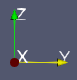
\includegraphics[width=3cm]{figures/axis_label.png}
	\caption{Axis orientation in all plots.} 
    \label{fig:axis}
\end{figure}
Also the contours of the surfaces have been coloured for easier destinction with the following colours:
\begin{itemize}
    \item \textbf{Red: }Mask
    \item \textbf{Yellow: }Substrate
    \item \textbf{Blue: }Passivation Layer
    \item \textbf{White: }If present corresponds to the initial configuration before any cycle.
\end{itemize}
 \subsubsection{Optimal Parameters}\label{sec:optimal_params}
 The best results were obtained with an \textbf{Deposition Time of $2.4$ s} and an \textbf{Etch Time of $6.7$ s}. This means a ratio $\lambda = \frac{t_{Etch}}{t_{Depos}} \approx 2.8$ is the optimal ratio between etch time and deposition time. The results can be seen in \autoref{fig:optimal_dir}. In this picture five cycles were simulated.
 \begin{figure}[H]
	\centering 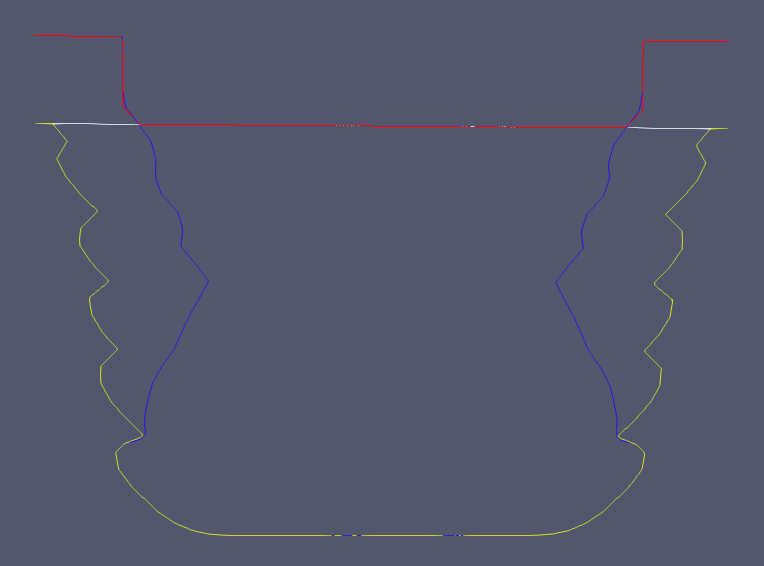
\includegraphics[width=9.5cm]{figures/optimal_dir.png}
	\caption{Perfect directional etching with optimal parameters.} 
    \label{fig:optimal_dir}
\end{figure}
It can be seen, that the passivation layer starts forming a cone (blue in \autoref{fig:optimal_dir}) which even closes the hole for large numbers of cycles. The reason for this is, that the etching is perfectly directional and at points of a normal vector z-component that is $\leq 0$ no etching takes place, which leads to accumulation due to the isotropic passivation layer growth. If the hole closes up during the cycles the process is broken. This can be seen in \autoref{fig:optimal_dir_long}.
 \begin{figure}[H]
	\centering 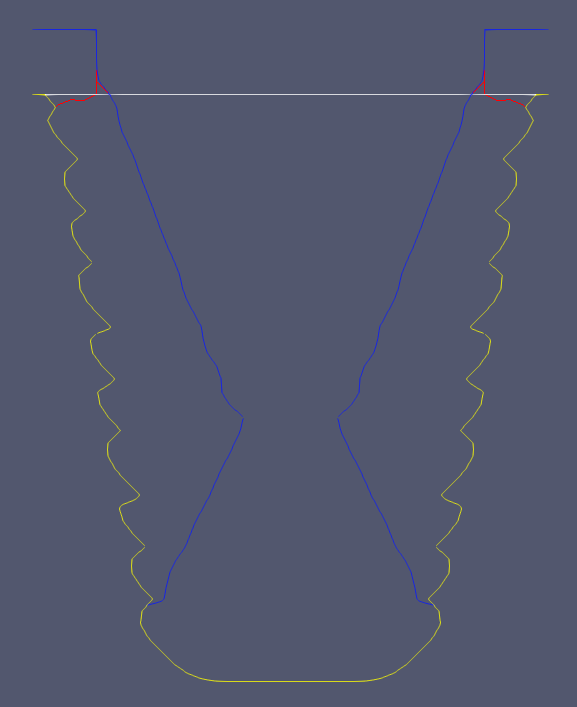
\includegraphics[width=9.5cm]{figures/optimal_dir_long.png}
	\caption{Optimal Parameters with ten cycles shows how the hole closes up.} 
    \label{fig:optimal_dir_long}
\end{figure}
 \begin{figure}[H]
	\centering 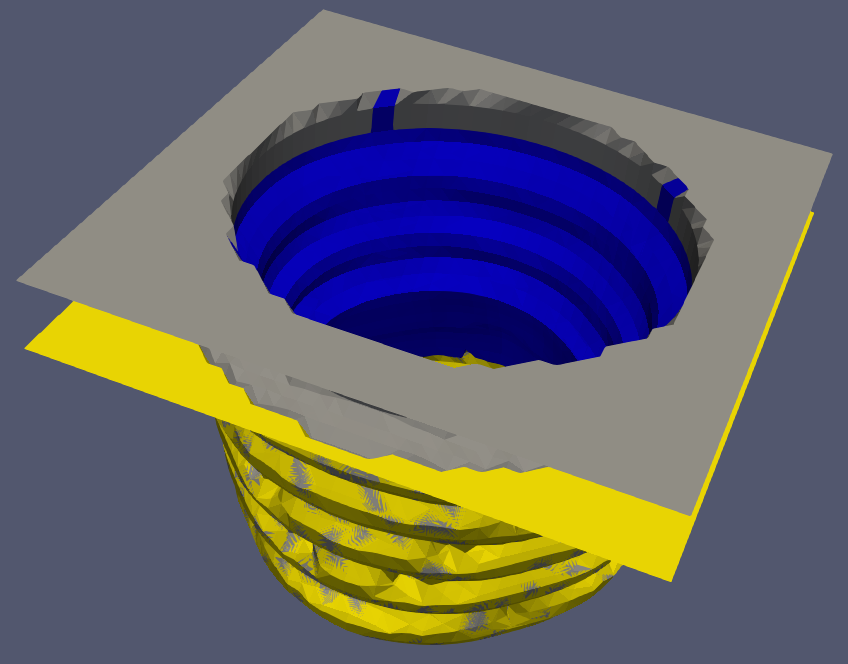
\includegraphics[width=9.5cm]{figures/3D_optimal_dir.png}
	\caption{3D rendering of the final configuration.} 
    \label{fig:3D}
\end{figure}

\subsubsection{Changing Parameters} \label{sec:Change_Params}
When changing the parameters of the etch and deposition times, one has to be careful, that the deposition time has to be shorter than the etch time. Otherwise the passivation layer is only 'scratched' in each cycle and the substrate is never touched.
For the rest of this subsection five cycles were used for better visualization.
In the following \autoref{fig:long_depos} the difference between deposition time and etch time is only one second ($3$s of deposition and $4$s of etch time). As can be seen this results in an almost cone shaped hole, due to the small amount of etching that takes place.
 \begin{figure}[H]
	\centering 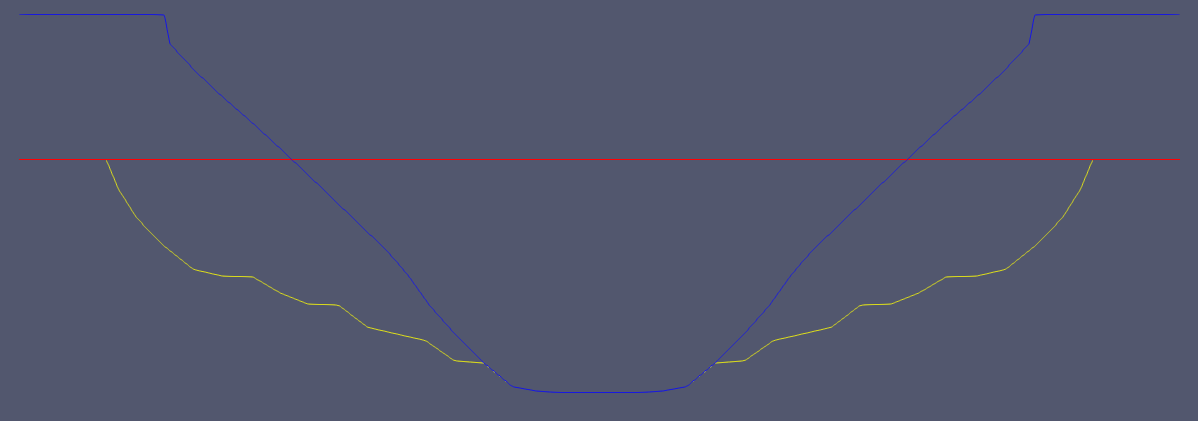
\includegraphics[width=9.5cm]{figures/longer_depos.png}
	\caption{Longer deposition time ($3$s and only $4$s of etch time).} 
    \label{fig:long_depos}
\end{figure}
In \autoref{fig:long_etch} the opposite is shown, where the etch time is way larger than the deposition time, which leads to very coarse scallops and a very uneven surface. In this example an deposition time of $2$s seconds and an etch time of $7$ seconds was used, because for larger differences the results are not visible inside the domain after the first cycle.
\begin{figure}[H]
	\centering 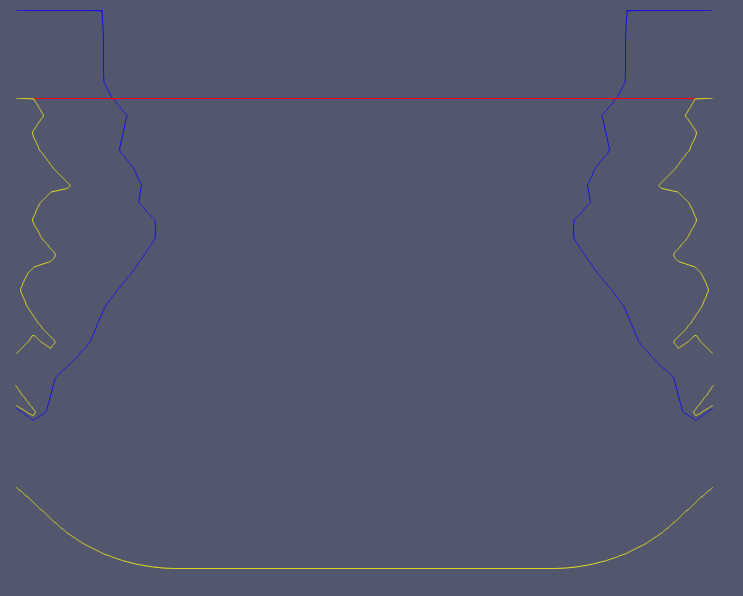
\includegraphics[width=9.5cm]{figures/longer_etch.png}
	\caption{Longer etch time ($2$s and only $7$s of etch time).} 
    \label{fig:long_etch}
\end{figure}
From the figures above one can see, that the larger the difference between the deposition and etch time, the more coarse the hole gets. This has the drawback of larger deviations horizontally and larger scallops. The benefit of this is faster 'drilling', meaning for the same depth less cycles are needed. This can lead to drastic cost reductions in the real fabrication scenario.\newline
If we look at the optimal parameters specified in \autoref{sec:optimal_params} the depts per cycle is approximately 3.8 to 4$\mu m$. This was measured using the ruler from paraview which is not exactly accurate. If we look at the $\lambda$ ratio from \autoref{sec:optimal_params} we can see, that the thickness per cycle can be expressed as:
\begin{align*}
    h = \lambda \cdot 1.4 = 2.8 \cdot 1.4 \approx 4
\end{align*}
It as to be kept in mind that this ratio is probably not consistent over the complete range of the possible $\lambda$s. Unfortunately due to time constraints no other $\lambda$s were inspected to find a more complex expression for the depth per etch $h$.
\subsubsection{Non Fully Directional Etch}\label{sec:dir_etch}
In this \autoref{sec:dir_etch} the effect of changing the directional etch to be more isotropic should be investigated. To achieve this inside the velocity layer the etch velocity is still proportional to the normal vector, but at least a minimum of $-0.3$.
\begin{lstlisting}
    if (normalVector[2] > 0) {velocity = -std::abs(normalVector[2]);} else {velocity = -0.3;}
\end{lstlisting}
This can be changed by commenting the corresponding lines 39 and 40 inside the code. The results can be seen in \autoref{fig:iso_etch_long}. The result looks a lot cleaner and more straight in the z-direction and is probably more realistic. But to get realistic values for the minimum etch rate in all directions would probably have to be determined through experiments.
 \begin{figure}[H]
	\centering 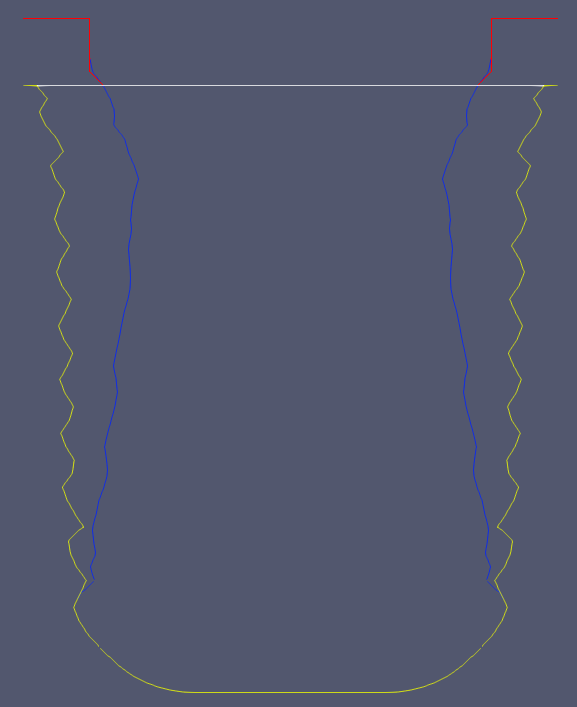
\includegraphics[width=7.5cm]{figures/optimal_iso_long.png}
	\caption{Ten cycles with more isotropic etching.} 
    \label{fig:iso_etch_long}
\end{figure}
\subsubsection{Scallop Size}
As \autoref{sec:Change_Params} already discussed, and shown the larger the difference between the deposition and etch time, the larger the scallops and horizontal deviation.

\section{Fin-FET Structure}


\end{document} 
